% f2000_spring_jingwan_science_q14_graph.tex — 2000 年·春季京皖卷·理科 第 14 题（f(x)=ax³+bx²+cx+d 的图象）
%
% 【来源】`.work/phase4-b20/source/2000春季京皖理.pdf`
%   （SHA-256 37f07244497aa0a21be12d8a31eac78b61490f835f088719a5990463585a35ce），
%   第 1 页（印刷页 61）；qpdf --qdf 解包后对内容流逐路径解析。
% 【坐标口径】源 PDF 用户空间（原点左下、y 向上）。本图本地坐标
%   (x, y) = (x_page − 608.528, y_page − 518.047)，1 单位 = 1 TeX pt；
%   O 取两轴交点；x 轴 y_page ≡ 518.047，y 轴 x_page ≡ 608.528。
% 【元素计数】5 条路径（x 轴／x 箭头／y 轴／y 箭头／曲线）＋ 5 个标签。
% 【标签】位置取 pdftotext -bbox 文本中心换算（源中心逐条记在 \node 行末）；
%   本图有 3 处微调（源位与微调量见各 \node 行末）：「O」左移 2.2 pt 避曲线，
%   「1」「2」同步下移 2.56 pt（保持两刻度同基线；「2」原净距仅 1.0 pt）。
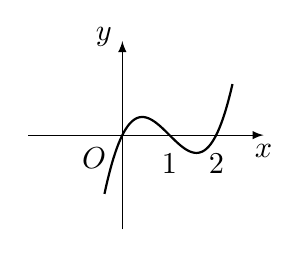
\begin{tikzpicture}[x=1pt, y=1pt,
    every node/.style={inner sep=0pt, font=\fontsize{10.5pt}{12.6pt}\selectfont}]
  \draw[line width=0.399pt] (-34.017,0) -- (47.438,0);
  \fill[line width=0.399pt] (51.025,0) .. controls (49.962,0.199) and (48.235,0.797) .. (47.04,1.494) -- (47.04,-1.494) .. controls (48.235,-0.797) and (49.962,-0.199) .. (51.025,0);
  \draw[line width=0.399pt] (0,-34.017) -- (0,30.43);
  \fill[line width=1.000pt] (0,34.016) .. controls (-0.199,32.954) and (-0.797,31.227) .. (-1.494,30.031) -- (1.494,30.031) .. controls (0.797,31.227) and (0.199,32.954) .. (0,34.016);
  % 曲线（本图第 5 条路径）：7177 个采样点 / 299 段三次贝塞尔。最小二乘拟合
  %   y = 0.003457x^3 - 0.176384x^2 + 1.999983x（rms 0.0002 pt，最大偏差 0.0025 pt），按该式绘制。
  \draw[line width=0.797pt, domain=-6.4632:39.7852, samples=240]
    plot (\x, {0.003457*\x*\x*\x - 0.176384*\x*\x + 1.999983*\x});

  \node[anchor=center] at (-6.648,35.403) {$y$};  % 源中心 (601.88,553.45)
  \node[anchor=center] at (-10.198,-8.247) {$O$};  % 源中心 (600.53,509.80)；左移 2.2 pt 避曲线（原净距 1.0 pt）
  \node[anchor=center] at (17.012,-10.397) {$1$};  % 源中心 (625.54,510.21)；与 2 同步下移 2.56 pt 保持同基线
  \node[anchor=center] at (34.012,-10.397) {$2$};  % 源中心 (642.54,510.21)；下移 2.56 pt 避曲线（原净距 1.0 pt）
  \node[anchor=center] at (51.022,-5.597) {$x$};  % 源中心 (659.55,512.45)
\end{tikzpicture}
%
% 【自验】
%   1) 探针编译：/tmp 最小文档（ctexart + common/preamble + xelatex）\input 本文件，0 error、0 warning。
%   2) 600 dpi 双渲染差分（有标签 / 标签 opacity=0）量测标签墨迹到路径墨迹最近距离：
%      各标签净距：「2」2.80、「x」2.85、「O」3.06、「1」4.35、「y」5.24 —— 最小 2.80 pt。
%   3) 线形：两轴 0.399 pt，曲线 0.797 pt，实线，与源 w 值一致；箭头为源贝塞尔填充路径。
%   4) 曲线拟合残差 rms 0.0002 pt、最大 0.0025 pt；根 x=0、17.00、34.02 与源标注 1、2 对位。
